\documentclass[14pt]{beamer} %Makes presentation
%\documentclass[handout]{beamer} %Makes Handouts
\usetheme{Singapore} %Gray with fade at top
\useoutertheme[subsection=false]{miniframes} %Supppress subsection in header
\useinnertheme{rectangles} %Itemize/Enumerate boxes
\usecolortheme{seagull} %Color theme
\usecolortheme{rose} %Inner color theme

\definecolor{light-gray}{gray}{0.75}
\definecolor{dark-gray}{gray}{0.55}
\setbeamercolor{item}{fg=light-gray}
\setbeamercolor{enumerate item}{fg=dark-gray}

\setbeamertemplate{navigation symbols}{}
%\setbeamertemplate{mini frames}[default]
\setbeamercovered{dynamics}
\setbeamerfont*{title}{size=\Large,series=\bfseries}

%\setbeameroption{notes on second screen} %Dual-Screen Notes
%\setbeameroption{show only notes} %Notes Output

\setbeamertemplate{frametitle}{\vspace{.5em}\bfseries\insertframetitle}
\newcommand{\heading}[1]{\noindent \textbf{#1}\\ \vspace{1em}}

\usepackage{bbding,color,multirow,times,ccaption,tabularx,graphicx,verbatim,booktabs,fixltx2e}
\usepackage{colortbl} %Table overlays
\usepackage[english]{babel}
\usepackage[latin1]{inputenc}
\usepackage[T1]{fontenc}
\usepackage{lmodern}

%\author[]{Thomas J. Leeper}
\institute[]{
  \inst{}%
  Department of Political Science and Government\\Aarhus University
}

\usepackage{tikz}
\usetikzlibrary{shapes,arrows}

\title{Ordinary Least Squares (Linear) Regression}

\date[]{February 17, 2015}

\begin{document}

\frame{\titlepage}

\frame{\tableofcontents}
% OLS
% Interpretation of coefficients
% Goodness-of-fit measures
% Standard errors, t-tests, p-values, and confidence intervals


\section{OLS}
\frame{\tableofcontents[currentsection]}

\frame{
	\frametitle{Uses of Regression}
	\begin{enumerate}\itemsep2em
	\item Description
	\item Prediction
	\item Causal Inference
	\end{enumerate}
}

\frame{
	\frametitle{Descriptive Inference}
	\begin{enumerate}
	\item We want to understand a \textit{population} of cases
	\item We cannot observe them all, so:
		\begin{enumerate}
    		\item Draw a \textit{representative} sample
    		\item Perform mathematical procedures on sample data
    		\item Use assumptions to make inferences about population
    		\item Express uncertainty about those inferences based on assumptions
		\end{enumerate}
	\end{enumerate}
}

\frame{
	\frametitle{Parameter Estimation}
	\begin{itemize}\itemsep1em
    	\item We want to observe population \textit{parameter} $\theta$
    	\item If we obtain a representative sample of population units:
    		\begin{itemize}
        		\item Our sample statistic $\hat{\theta}$ is an unbiased estimate of $\theta$
        		\item Our sampling procedure dictates how uncertain we are about the value of $\theta$
    		\end{itemize}
	\end{itemize}
}

\frame{
	\frametitle{Sample Estimate of Population Mean}
	We want to know $Y$ (population mean)\\
	Our \textit{estimator} is the sample mean formula which produces the sample \textit{estimate} $\bar{y}$:
	\begin{equation}
	\bar{y} = \frac{1}{n}\sum_{i=1}^{n}y_i
	\end{equation}
	where $y_i = $ value for a unit, and\\
	$n = $ sample size
	
	\begin{equation}
	SE_{\bar{y}} = \sqrt{(1-f)\frac{s^2}{n}}
	\end{equation}
	where $f = $ proportion of population sampled,\\
	$s^2 = $ sample element variance, and\\
	$n = $ sample size
}

\frame{
	\frametitle{Uncertainty}
	\begin{itemize}\itemsep1em
		\item We never know $\theta$
		\item $\hat{\theta}$ is an estimate that may not equal $\theta$
			\begin{itemize}
    			\item Unbiased due to \textbf{Law of Large Numbers}
    			\item For $\bar{y}$: $N(Y, \sigma^2) $
			\end{itemize}
    	\item The size of $SE_{\bar{\theta}}$ depends on:
    		\begin{itemize}
        		\item Element variance
        		\item Sample size
    		\end{itemize}
    	\item We may want to know $\hat{\theta}$ per se, but we are mostly interested in it as an estimate of $\theta$
	\end{itemize}
}

\frame{
	\frametitle{Causal Inference}
	\begin{enumerate}\itemsep1em
	\item<2-> Everything that goes into descriptive inference
	\item<3-> Plus, philosophical assumptions
	\item<4-> Plus, randomization \textit{or} perfectly specified model
	\end{enumerate}
}



% OLS equation

\frame{
	\frametitle{Bivariate Regression I}
	\begin{itemize}\itemsep1em
	\item $Y$ is continuous
	\item $X$ is a randomized treatment indicator/dummy $(0,1)$
	\item How do we know if the treatment $X$ had an effect on $Y$?
	\item<2-> Look at mean-difference: $E[Y_i|X=1] - E[Y_i|X=0]$
	\end{itemize}
}



\frame<1-2>[label=dummy]{
	\frametitle{Bivariate Regression II}
	\begin{itemize}\itemsep1em
    	\item Mean $E[Y_i|X=1] - E[Y_i|X=0]$ is the regression line slope
    	\item Slope ($\beta$) defined as $\frac{\delta Y}{\delta X}$
    		\begin{itemize}
        		\item<2-> $\delta Y = E[Y_i|X=1] - E[Y_i|X=0]$
        		\item<2-> $\delta Y = 1 - 0 = 1$
    		\end{itemize}
    	\item<3-> How do we know if this is a \textit{significant} difference?
    		\begin{itemize}
        		\item We'll come back to that
    		\end{itemize}
	\end{itemize}

}

% graphs of mean-difference
% http://thomasleeper.com/regcourse/Slides-2014/Session02_01.html#20


\frame{
	\begin{center}
	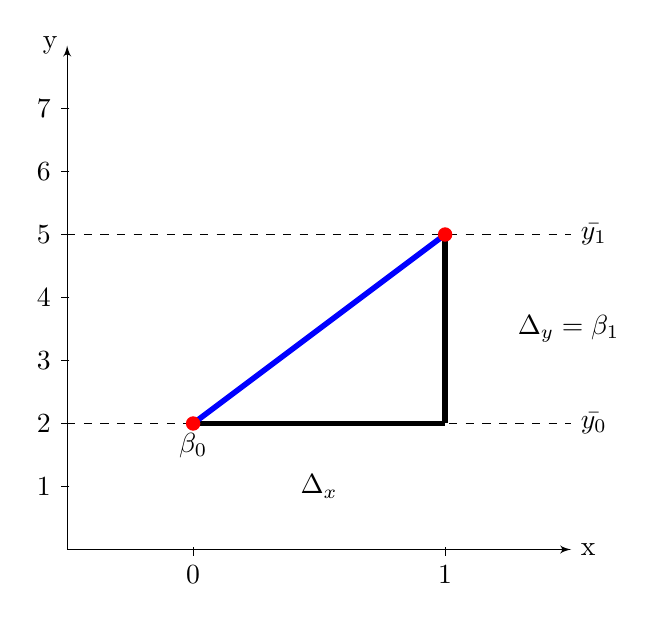
\begin{tikzpicture}[>=latex', scale=0.8]
        \draw[->] (0,0) node[below] (origin) {}  -- (8,0) node[right] (xaxis) {x};
        \draw[->] (origin) -- (0,8) node[left] (yaxis) {y};
        % x ticks
        \draw (2,1pt) -- (2,-3pt) node[anchor=north] {0};
        \draw (6,1pt) -- (6,-3pt) node[anchor=north] {1};
        % y ticks
        \foreach \y in {1,...,7}
             \draw (1pt,\y) -- (-3pt,\y) node[anchor=east] {$\y$};
        
        % points
        
        
        % y_0-bar
        \draw[dashed] (0,2) -- (8,2) node[right] {$\bar{y_0}$};
        % y_1-bar
        \draw[dashed] (0,5) -- (8,5) node[right] {$\bar{y_1}$};
        
        % slope
        \draw[solid, line width=2pt] (2,2) -- (6,2);
        \draw[solid, line width=2pt] (6,2) -- (6,5);
        \node(deltax) at (4,1) {$\Delta_x$};
        \node[right](deltay) at (7,3.5) {$\Delta_y = \beta_1$};
        
        \draw[blue, solid, line width=2pt] (2,2) -- (6,5);
        \node[below](b0) at (2,2) {$\beta_0$};
        
        % mean points
        \draw[red,fill] (2,2) circle [radius=3pt];
        \draw[red,fill] (6,5) circle [radius=3pt];
                
    \end{tikzpicture}
    \end{center}
}



\frame{
	\begin{center}
	\begin{tikzpicture}[>=latex', scale=0.8]
        \draw[->] (0,0) node[below] (origin) {0}  -- (8,0) node[right] (xaxis) {x};
        \draw[->] (origin) -- (0,8) node[left] (yaxis) {y};
        % x ticks
        \foreach \x in {1,...,7}
        	\draw (\x,1pt) -- (\x,-3pt) node[anchor=north] {$\x$};
        % y ticks
        \foreach \y in {1,...,7}
             \draw (1pt,\y) -- (-3pt,\y) node[anchor=east] {$\y$};
        % points
        \draw[fill] (1,2) circle [radius=1.5pt];
        \draw[fill] (2,5) circle [radius=1.5pt];
        \draw[fill] (3,3) circle [radius=1.5pt];
        \draw[fill] (4,5) circle [radius=1.5pt];
        \draw[fill] (5,2) circle [radius=1.5pt];
        \draw[fill] (6,7) circle [radius=1.5pt];
        % x-bar
        \draw[dashed] (3.5, 0) -- (3.5,8) node[above] {$\bar{x}$};
        % y-bar
        \draw[dashed] (0,4) -- (8,4) node[right] {$\bar{y}$};
    \end{tikzpicture}
    \end{center}
}

\begin{comment}

| x | y |
| ---- | ---- |
| 1 | 2 |
| 2 | 5 |
| 3 | 3 |
| 4 | 5 |
| 5 | 2 |
| 6 | 7 |
| `\(\bar{x}=?\)` | `\(\bar{y}=?\)` |
| `\(\bar{x}=3.5\)` | `\(\bar{y}=4\)` |
`\(\beta_1 = \frac{\Sigma(x_i-\bar{x})(y_i-\bar{y})}{\Sigma(x_i-\bar{x})^2} = ?\)`
`\( \beta_0 = \bar{y} - (\beta_1 * \bar{x}) = 4 - (0.6857 * 3.5) =  \)`

\end{comment}

\againframe<2-3>{dummy}


\frame{
	\frametitle{Systematic versus unsystematic component of the data}
	\begin{itemize}
    	\item Regression line (slope) is the systematic component
    	\item Linear regression fits the conditional mean of the data (i.e., $E[Y|X=x]$)
    	\item Error term is the deviation of observations from the line (i.e., the unsystematic, unexplained part)
    		\begin{itemize}
        		\item The difference between each value $Y_i$ and $E[Y|X=X_i]$ is the \textit{residual}: $\epsilon_i$
        		\item OLS produces an estimate of the relationship between X and Y that minimizes the residual sum of squares
    		\end{itemize}
    	\item Why are there residuals?
    		\begin{itemize}
    		\item Omitted variables
    		\item Measurement error
    		\item Fundamental randomness
    		\end{itemize}
	\end{itemize}
}

\frame{
	\frametitle{Ways of Thinking About OLS}
	\begin{enumerate}
    	\item Estimating Unit-level Causal Effect
    	\item Minimizing residual sum of squares (RSS)
    	\item Ratio of $Cov(X,Y)$ and $Var(X)$
	\end{enumerate}
}

% equations: unit, sample, population



% graphs
% sum of squares total
% regression sum of squares
% sum of squares residuals or sum of squared errors


\begin{comment}


% $\frac{Cov(X,Y)}{Var(X)}$
% define variance and covariance
% Requirements: variation in X ($\beta$ undefined)
% Requirements: variation in Y? (No, answer is 0)
% Requirements: $N \ge k$, where $k$ is number of parameters to be estimated
% Multivariate context requires more complex formula involving matrices (Angrist and Pischke); Week 20


% Is this any good?
% works mathematically; X is measured without error; linear relationship


OLS is BLUE due to the Gauss-Markov assumptions
   1. Linearity in parameters
   2. Random sampling
   3. No collinearity
   4. Expected value of errors is zero
   5. Homoskedasticity


Least Squares versus Least Absolute Deviations
 - Both are unbiased estimates of the population regression line
 - OLS is more efficient (small variance)
 - Thus OLS is BLUE



Endogeneity
 Measurement error in regressors
 Omitted variables associated with included regressors (``specification error'')
   -> including irrelevant variable is unproblematic, but may cost precision
 Lack of temporal precedence

Omitted variables
Measurement error
 Independent variables
  $y = \beta_0 + \beta_1 x* + \epsilon$
  $x = x* + w$
  $y = \beta_0 + \beta_1 x + (\epsilon - \beta_1 w) = \beta_0 + \beta_1 x + v$
  Attenuation: as measurement error increases, estimated effect goes to zero; all other $\beta$ are also biased in unknown directions
 Dependent variables
   - If random (i.e., uncorrelated with $X$, costs us precision)
   - If systematic, who knows what consequences it has
   - Special case: Censoring, something we'll deal with in Lectures 11 and 12
Posttreatment bias
Multicollinearity
 - Perfect multicollinearity: equation not estimable
 - High correlation among X's: drop one or more regressors
Missing data
 - Problem
 - Deal with it in Lecture 5


\frame{
	\begin{center}
	\begin{tikzpicture}[>=latex',circ/.style={draw, shape=circle, node distance=5cm, line width=1.5pt}]
        \draw[->] (0,0) node[left] (X) {X} -- (5,0) node[right] (Y) {Y};
        \draw[->] (0,0) node[left] (X) {X} -- (2.5,0) node[right] (D) {D};
        \draw[->] (3.1,0) -- (5,0) node[right] (Y) {Y};
        \draw[->] (-3,4) node[above] (Z) {Z} -- (X);
        \draw[->] (Z) -- (Y);
        \draw[->] (5,2) node[above] (A) {A} -- (Y);
        \draw[->] (-2,0) node[left] (B) {B} -- (X);
        \draw[->] (X) -- (2,-2) node[right] (C) {C};
    \end{tikzpicture}
    \end{center}
}




\frame{
	\frametitle{Post-treatment Bias}
	\begin{itemize}
	\item We usually want to know the \textbf{total effect} of a cause
	\item If we include a mediator, $M$, of the $X \rightarrow Y$ relationship, the coefficient on $X$:
		\begin{itemize}
    		\item Only reflects the \textbf{direct} effect
    		\item Excludes the \textbf{indirect} effect of $X$ through $M$
		\end{itemize}
	\item So don't control for mediators!
	\end{itemize}
}
% Goodness of fit
% correlation: $cor(x,y) = \hat{r}_{x,y} = \frac{cov(x,y)}{(n-1)sd(x)sd(y)}$
	% Slope $\hat{\beta}_1$ and correlation $\hat{r}_{x,y}$ are simply different scalings of $cov(x,y)$
	% Correlation tells us how well the bivariate relationship is summarized by a cloud of points
	% Slope tells us the expected change in `\(y\)` given a unit change in `\(x\)`
% $R^2 = cor(x,y)^2 = \frac{SSE}{SST} = 1 - \frac{SSR}{SST}$
	% increases simply by adding more variables
	% $Adj.R^2 = R^2 - (1 - R^2)\frac{k}{n-k-1}$, where $k$ is number of regressors
	% unitless
% $\sigma$
	% Standard Error of the Regression (SER) or Root Mean Squared Error (RMSE)
	% How far, on average, are the observed $y$ values from their corresponding fitted values $\hat{y}$
	% $\hat{\sigma} = \sqrt{\frac{RSS}{n-p}}$, where $p$ is number of parameters estimated
	% Think about how before modelling $\bar{y}$ is our best estimate of $y$ for any $x$
	% $sd(y)$ is how far, on average, a given observation is from our estimate of its value
	% same units as $y$; always smaller than $sd(y)$
% F-test
	% Omnibus test of whether any of our coefficients differ from zero
	% In a bivariate regression, `\(F=t^2\)`
	% unitless; not a very interesting test of anything
	% nested model comparison
		F-test for comparing two nested models
		   - Reduced model: `\( \hat{y} = \hat{\beta_0} + \hat{\beta_1}x_1 \)`
		   - Expanded model: `\( \hat{y} = \hat{\beta_0} + \hat{\beta_1}x_1 + \hat{\beta_2}x_2 + \dots \)`
		
		 - "Reduced" model is nested within the expanded model
		
		 - The F-test comparing the two models tells us if the expanded model significantly reduces RSS

\frame{
\begin{alltt}
. reg growth lcon

      Source |       SS       df       MS              Number of obs =      44
-------------+------------------------------           F(  1,    42) =    0.09
       Model |  .000038348     1  .000038348           Prob > F      =  0.7615
    Residual |  .017255198    42  .000410838           R-squared     =  0.0022
-------------+------------------------------           Adj R-squared = -0.0215
       Total |  .017293546    43  .000402175           Root MSE      =  .02027

------------------------------------------------------------------------------
      growth |      Coef.   Std. Err.      t    P>|t|     [95% Conf. Interval]
-------------+----------------------------------------------------------------
        lcon |  -.0017819   .0058325    -0.31   0.761    -.0135524    .0099886
       _cons |   .0158988   .0390155     0.41   0.686    -.0628376    .0946353
------------------------------------------------------------------------------
\end{alltt}
}

\frame{
\begin{alltt}
. nestreg: reg growth lcon (lconsq)

+-------------------------------------------------------------+
                Block  Residual                     Change 
Block        F     df        df   Pr > F       R2    in R2 
-------+-----------------------------------------------------
1         0.09      1        42   0.7615   0.0022          
2         7.98      1        41   0.0073   0.1649   0.1626 
+-------------------------------------------------------------+
\end{alltt}
}


% types of variables
% interval
% indicator
% categorical
% ordinal

Two things to keep in mind:

 - Effect `\(\beta_1\)` is constant across values of X1
 
 - Effect is *also* constant across values of other covariates
 
 - This all changes when we have:
   1. Interaction terms
   2. Nonlinear covariates (e.g., `\(x^2\)`)
   2. Models other than OLS

Our interpretations are sample-level interpretations
    - We need to have a representative sample to make population-level inferences
    - But we rarely have truly representative samples
  
  - Uncertainty means coefficients in model are unlikely to be exactly the population-level ("true") effects
    - Better not to think about the point estimates (slopes) but instead the interval






\frame{
	\frametitle{What goes in our regression?}
	\begin{itemize}\itemsep1em
    	\item Use theory to build causal models
    	\item Often, a causal graph helps
    	\item Use empirical correlations to add additional ``controls''
	\end{itemize}
}

\frame{
	\frametitle{Common Conditioning Strategies}
	\begin{enumerate}\itemsep1em
    	\item Condition on nothing (``naive effect'')
    	\item Condition on some variables
    	\item Condition on observables
	\end{enumerate}
}

\frame{
	\begin{center}
	\begin{tikzpicture}[>=latex',circ/.style={draw, shape=circle, node distance=5cm, line width=1.5pt}]
        \draw[->] (0,0) node[left] (X) {X} -- (5,0) node[right] (Y) {Y};
        \draw[->] (0,0) node[left] (X) {X} -- (2.5,0) node[right] (D) {D};
        \draw[->] (3.1,0) -- (5,0) node[right] (Y) {Y};
        \draw[->] (-3,4) node[above] (Z) {Z} -- (X);
        \draw[->] (Z) -- (Y);
        \draw[->] (5,2) node[above] (A) {A} -- (Y);
        \draw[->] (-2,0) node[left] (B) {B} -- (X);
        \draw[->] (X) -- (2,-2) node[right] (C) {C};
    \end{tikzpicture}
    \end{center}
}


% multivariate regression interpretation





\frame{
	\frametitle{Significance}
	\begin{enumerate}\itemsep2em
    	\item Substantive significance
    		\begin{itemize}
        		\item<2-> Is the effect size \textit{important} in the real world?
    		\end{itemize}
    	\item Statistical significance
    		\begin{itemize}
        		\item<3-> Is the effect size larger than a predetermined threshold?
    		\end{itemize}
	\end{enumerate}
}

% To draw inferences about the population, we need to account for uncertainty in our estimates
% We do this by generating standard errors (SEs) for the regression estimates

% SEs
	% Definition: The standard error of a sample estimate is the average distance that a sample estimate would be from the population value if we drew lots and lots of separate random samples.
	% If we repeated our sampling procedure an infinite number of times, the SE is the average deviation of a sample estimate from the population mean
	% Standard errors are based on assumptions about the sampling process, not anything about our sample data per se
	
	
SE Interpretation

  - SE is a ratio of unexplained variance in `\(y\)` (weighted by sample size) and variance in `\(x\)`

  - More variance in `\(x\)` means smaller SE

  - More unexplained variance in `\(y\)` means bigger SE

  - More observations yields smaller numerator in `\(s_{\hat{\beta_1}}\)`, meaning smaller SE

  - The SE has the units of the coefficient (i.e., `\(y\)` per `\(x\)`))
  
  $var(\hat{\beta_1}) = \frac{\frac{1}{n-2}RSS}{SS_x}$
  $s_{\hat{\beta_1}} = \sqrt{\frac{\frac{1}{n-2}RSS}{SS_x}} = \sqrt{\frac{\sigma^2}{SS_x}}$
  % more complicated in a multivariate regression
  
  
## Homoskedasticity and heteroskedasticity

  - The basic SE formula (and the default calculations in Stata) assume homoskedasticity
  
  - When errors are heteroskedastic, we need ``robust'' SEs

  - David will cover this in Lecture 4

% assumption of Normality
% $y|x \sim N(\beta_0 + \beta_1x_1 + ..., \sigma^2)$
% There is a population of identically distributed cases of which our data are one sample

% t-statistics
% regression on population versus sample versus super-population
% The sampling distribution for `\(\beta_1\)` that we just assumed (partially based on our data), allows us to conduct hypothesis tests
% The kinds of hypotheses we can test are of the form:
	% Bivariate: ``$X$ has no effect on $Y$''
	% Multivariate: ``accounting for the other variables in the model, $X$ has no effect on the expected value of $Y$''

% often use a no-effect null hypothesis, but we can do anything
% $\frac{\hat{\beta_1} - \alpha}{SE_{\hat{\beta_1}}}$, where $\alpha$ is our null hypothesis value

% - The $t$*-statistic from a $t$-test of mean-difference is the same as the $t$-statistic from a $t$-test on an OLS slope for a dummy covariate
% $t_{\hat{\beta_1}} = \frac{\hat{\beta_1}}{SE_{\hat{\beta_1}}}$
% we then go back to the $t$-distribution function (which tells us how likely a given $t$-ratio is)

% The p-value is the probability of seeing a t-ratio/t-statistic as large or larger than the one we observed in our data

Definition of p-value:

the probability of a *t*-statistic as extreme as the one we observed, if the null hypothesis was true

the probability of a slope as large as the one we observed, given the observed variance in the data and that the null hypothesis was true


The p-value is not:

  - The probability that a hypothesis is true or false

  - A reflection of our confidence or certainty about the result

  - The probability that the true slope is in any particular range of values

  - A statement about the importance or substantive size of the effect
  
  
A CI is simply a range, centered on the slope
CIs and p-values convey the same information
CIs are on the scale of the statistic of interest (and thus the scale of the original data)
If the confidence interval overlaps zero, we would be unable to reject the null the hypothesis

Definition: Were we to repeat our procedure of sampling, analyzing the sample, and calculating a confidence interval *repeatedly* from the population, a fixed percentage of the resulting intervals would include the true population-level slope.

We cannot say for sure whether the estimated confidence interval *this time* actually includes that true slope



\end{comment}



\appendix
\frame{}

\end{document}
